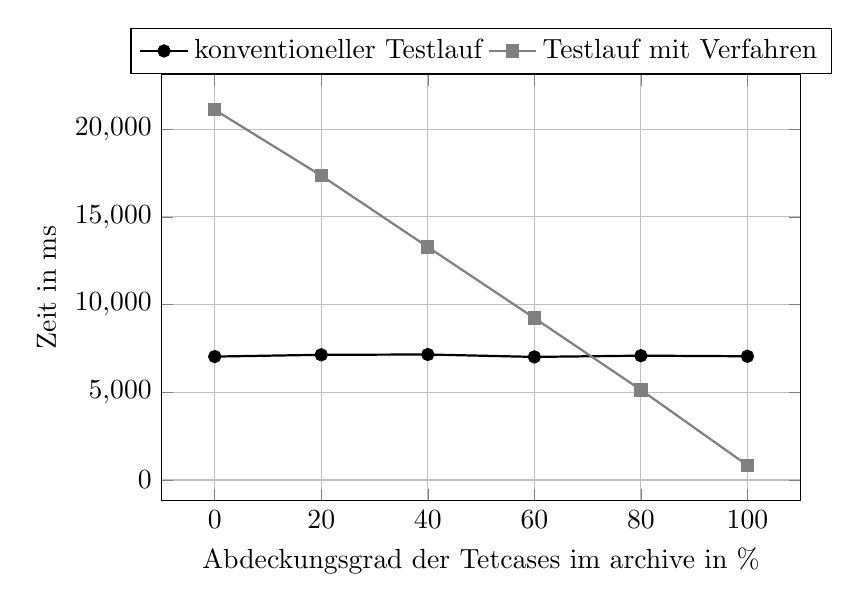
\begin{tikzpicture}
    \begin{axis}[
        width=0.8\textwidth,
        height=7cm,
        xlabel={Abdeckungsgrad der Tetcases im archive in \%},
        ylabel={Zeit in ms},
        grid=major,
        scaled y ticks=false,
        yticklabel style={
            /pgf/number format/fixed,
            /pgf/number format/precision=0
        },
        legend style={
            at={(0.5,1.0)},
            anchor=south,
            legend columns=2
        }
    ]
    \addplot[
        thick,
        mark=*,
    ] coordinates {
        (0, 7036.4)
        (20, 7137.5)
        (40, 7154.3)
        (60, 7017.1)
        (80, 7087.7)
        (100, 7054.8)
    };
    \addlegendentry{konventioneller Testlauf}
    \addplot[
        thick,
        mark=square*,
        gray!100,
    ] coordinates {
        (0, 21107.8)
        (20, 17356.5)
        (40, 13287.1)
        (60, 9234.9)
        (80, 5136.3)
        (100, 830.7)
    };
    \addlegendentry{Testlauf mit Verfahren}
    \end{axis}
\end{tikzpicture}
